\documentclass{emulateapj}
\bibliographystyle{apj}

%define general packages
\usepackage{epsfig}
\usepackage{rotating}
\usepackage{amsmath}
\usepackage{natbib}
\usepackage{footnote}
\usepackage{courier}

%internal short cuts
\def \HgA {H$\gamma_A$}
\def \Hbp {H$\beta ^\prime$}

\begin{document}

\title{PRIMUS: Galaxy Environment on the Quiescent Fraction Evolution at $z < 1$}
\author{ChangHoon Hahn, Michael Blanton, Alison Coil, Richard Cool, Daniel Eisenstein, John Moustakas, Ken Wong, Guangtun Zhu}

\begin{abstract}
We investigate the effects of galaxy environment on the evolution of the quiescent fraction ($f_{\rm{Q}}$) from $z =0.8 $ to $ 0.0$ using spectroscopic redshifts and multi-wavelength imaging data from PRism MUlti-object Survey (PRIMUS) and the Sloan Digitial Sky Survey (SDSS). Our stellar mass limited galaxy sample consists of $\sim 40000$ PRIMUS galaxies within $z = 0.2-0.8$ and $\sim 130000$ SDSS galaxies within $z = 0.0375-0.145$. We classify the galaxies as quiescent or star-forming, based on an evolving specific star formation cut, and as low or high density environments, based on fixed cylindrical aperture environment measurements on a volume-limited {\em Environment Definition Population} (from PRIMUS and SDSS). 

For each of these subsamples, we examine the stellar mass function (SMF) evolution and compute the $f_{\rm{Q}}(\mathcal{M}_{*})$. We find that in both low and high density environments the quiescent fraction increases with cosmic time over the probed redshift range. Moreover, the difference between the quiescent fraction in low and high density environments remains constant throughout the redshift range. These results suggest that the evolution of the quiescent fraction is independent of environment and provide constraints on quenching mechanisms in high density environments such as groups and clusters.  
\end{abstract}

%Section `ing
\section{Introduction}
Galaxies, in their detailed properties, carry the imprints of their
surroundings, with a strong dependence of the quiescent fraction of
galaxies on their local environment (e.g. \citealt{hubble36a,
oemler74a, dressler80a, hermit96a, guzzo97a}; for a recent review see
\citealt{blanton09a}).  The strength of this dependence is itself a
strongly decreasing function of galaxy stellar mass; at the extreme,
the lowest masses ($<10^{9}$ $M_\odot$) galaxies are quenched only in
dense regions, and never in isolation (\citealt{geha12a}).  These
effects vary with redshift at least in the densest clusters, as
observed in the changing fraction of late-type spirals relative to the
field found in studies of the morphology-density relation
(\citealt{dressler84a, desai07a}).  Clearly understanding the
properties of galaxies in the present-day universe requires a careful
investigation of the role of environment, and how that role changes
over time.

Nevertheless, the evolution of the role of environment is a relatively
subtle effect and difficult to study.  Although history of galaxies
prior to $z\sim 1$ appears to have been one of rapid assembly, since
that time the galaxy population has continued to evolve, but less
dramatically. Although there are detectable changes in the population,
the major classes of galaxies existed at $z\sim 1$, in roughly the
same relative numbers as today (\citealt{bundy06a, borch06a,
taylor09a, moustakas13a}. Furthermore, at those redshifts we can also
detect the dependence of galaxy properties on environment, with lower
star-formation rate early-type galaxies populating the denser regions
(\citealt{cooper08a, patel09a, kovac10a}).

The most dramatic change in galaxy properties during the past eight
billion years has been a remarkable decline in the star-formation rate
of galaxies in the Universe (\citealt{hopkins06a}).  This decline
appears dominated by decreases in the rates of star-formation of
individual galaxies (\cite{Noeske:2007aa}). There is evidence that a
large fraction of the decline associated with strongly
infrared-emitting starbursts (\citealt{bell05a, magnelli09a}).  The
decline does not appear to be due to the quenching of a large
fractions of the star-forming population, as reflected in observations
of the stellar mass function of quiescent and star-forming galaxies
(\cite{Blanton:2006aa},\citealt{bundy06a, borch06a, moustakas13a}).  These
findings leave little room for the participation of
environmentally-driven quenching in the global census of
star-formation.  As \citet{cooper08a} and others have pointed out,
because the environmental dependence of total star-formation rates at
fixed redshift is relatively small, environmentally effects are
unlikely to cause the overall star-formation rate decline.

Thus, the impact of environment on galaxy formation has to be
interpreted on top of the background of this overall decline affecting
galaxies in all environments.  The most straightforward investigation
of would directly determine the star-forming properties of galaxies as
a function of environment, stellar mass and redshift in a single,
consistently analyzed data set. This analysis can reveal how galaxies
are quenched in the universe over time, quantitatively establish the
contribution of environmental effects to the overall trends, and
reveal whether those trends happen equally in all environments.
However, such an analysis has not been done previously due to the lack
of sufficiently large samples. In this paper, we apply this approach
using the Prism Multi-object Survey (PRIMUS; \cite{Coil:2011aa}, 
\cite{Cool:2013aa}), the largest available redshift survey covering the epochs
between $0<z<1$.

In Section \ref{sec:sample} we present a brief description of the PRIMUS and SDSS data, our sample construction, and galaxy environment measurements. In Section \ref{sec:smf} we examine the stellar mass function evolution for star-forming/quiescent and high/low density environment subsamples. In Section \ref{sec:qf_const} we compare the quiescent fraction evolution for high and low density environments and discuss implications of the results on quenching mechanisms. In Section \ref{sec:summary} we summarize our results. 

Throughout the paper we assume cosmology with $\Omega_{m} = 0.3, \Omega_{\Lambda} = 0.7$, and $H_0 = 70 \rm{km} \; \rm{s}^{-1} \rm{Mpc}^{-1}$.

\section{Sample Selection} \label{sec:sample}
In order to quantify the effects of galaxy environment on the evolution of the quenched population over the redshift range $z < 1.0$, we require a sample with sufficient depth and robustness to probe the redshift range and to measure galaxy environment. PRIMUS with its $\sim 120,000$ spectroscopic redshifts provides ideal data at intermediate redshifts for our analysis. In addition, we anchor our analysis of the intermediate redshift sample with a low redshift sample derived from SDSS. 

In Section \ref{sec:primus} and Section \ref{sec:sdss} we provide a brief summary of the PRIMUS data and the SDSS data used for our sample selection. Then in Section \ref{sec:target} we define our stellar mass complete galaxy sample. Afterwards, in Section \ref{sec:sfq}, we classify our sample galaxies as quiescent or star-forming then calculate the environment using a volume-limited {\em Environment Defining Population} in Section \ref{sec:environment}. 
Finally in Section \ref{sec:edgeeffect}, we correct our galaxy sample and environment measurements for edge effects of the surveys. 

\subsection{PRIMUS} \label{sec:primus}
For our sample at intermediate redshifts we use multiwavelength imaging and spectroscopic redshifts from PRIMUS, a faint galaxy survey with $\sim 120,000$ precise spectroscopic redshifts ($\sigma_z/(1+z) \approx 0.5 \%$) within the range $z \approx 0-1.2$. The survey was conducted using a IMACS spectrograph on a Magellan I Baade $6.5$ m telescope with a slitmask and low dispersion prism. For details on the PRIMUS observation methods such as survey design, targeting, and data summary, we refer readers to the survey papers: \cite{Coil:2011aa} and \cite{Cool:2013aa}. 

While the PRIMUS survey targeted seven distinct extragalactic deep fields for a total of $\sim 9 \; \rm{deg}^2$, we restrict our sample to five fields that have $GALEX$ and {\em Spitzer}/IRAC imaging (similar to the sample selection in \cite{Moustakas:2013aa}). Four of these fields are a part of the {\em Spitzer} Wide-area Infrared Extragalactic Survey (SWIRE\footnote{http://swire.ipac.caltech.edu/swire/swire.html} ): the European Large Area ISO Survey - South $1$ field (ELAIS-S1\footnote{http://dipastro.pd.astro.it/esis}), the Chanddra Deep Field South SWIRE field (CDFS), and the XMM Large Scale Structure Survey field (XMM-LSS). The XMM-LSS consists of two separate but spatially adjacent fields: the Subaru/XMM-Newton DEEP Survey fied (XMM-SXDSS\footnote{http://www.naoj.org/cience/SubaruProject/SDS}) and the Canadian-France-Hawaii Telescope Legacy Survey field (XMM-CFHTLS\footnote{http://www.cfht.hawaii.edu/Science/CFHLS}). Our fifth and final field is the Cosmic Evolution Survey (COSMOS\footnote{http://cosmos.astro.caltech.edu}) field. For all of our fields we have near-UV (NUV) and far-UV (FUV) photometry from the {\em GALEX} Deep Imaging Survey (DIS; \cite{Martin:2005aa}; \cite{Morrissey:2005aa}) as well as ground-based optical and {\em Spitzer}/IRAC mid-infrared photometric catalogs. \cite{Moustakas:2013aa} provides detailed descriptions of integrated flux calculations in the photometric bands for each of our fields. 

Finally, from the spectroscopic redshift and broad wavelength photometry we use \texttt{iSEDfit}, a Bayesian SED modeling code, to calculate stellar masses and star formation rates (SFRs) for our sample galaxies. \texttt{iSEDfit}, uses the redshift and the observed photometry of the galaxies to determine the statistical likelihood of a large ensemble of generated model SEDs. The model SEDs are generated using Flexible Stellar Population Synthesis (FSPS) models (\cite{Conroy:2010aa}) based on \cite{Chabrier:2003aa} IMF, along with other prior parameters beyond the scope of this paper. For details we refer readers to Section 4.1 and Appendix A. of \cite{Moustakas:2013aa}. For the observed photometry, we use the {\em GALEX} FUV and NUV, the two shortest IRAC bands at $3.6$ and $4.5 \mu \rm{m}$ (the two longer-wavelength IRAC channels are excluded because \texttt{iSEDfit} does not model hot dust or polycyclic aromatic hydrocarbons emission lines), and the optical bands. 

\begin{table} %Subject to significant change based on the classification of environment
  \caption{Galaxy Subsamples}
  \label{tab:subsample}
  \begin{center}
    \leavevmode
    \begin{tabular}{lllll} \hline \hline              
    $z$ &Environment        &Quiescent  &Star-forming  \\ \hline 
$0.0375-0.145$ &High           &5470                       &4501                           \\
               &Low            &5419                       &8927                           \\
               &               &                       &                           \\ \hline
$0.2-0.4$      &High           &322                    &583                           \\
               &Low            &768                    &2516                           \\
               &               &                       &                           \\ \hline
$0.4-0.6$      &High           &350                       &675                           \\
               &Low            &871                       &2385                           \\
               &               &                       &                           \\ \hline
$0.6-0.8$      &High           &347                       &430                           \\
               &Low            &833                       &1847                           \\
               &               &                       &                           \\ \hline
  \multicolumn{4}{l}{}                                             \\       
    \end{tabular} 
  \end{center}
\end{table}

\begin{figure*}
    \begin{center}
        \leavevmode
        \epsscale{1.2}
	\plotone{fig_edp_sdss_z005_012_primus_z02_10_Mr_redshift.png}
        \caption{Absolute magnitude $M_{r}$ versus redshift for the target galaxy population (black squares) with the Environment Defining Population (red circles) plotted on top. Both samples are divided into redshift bins:$z \approx 0.0375-0.145$, $0.2-0.4$, $0.4-0.6$, and $0.6-0.8$ (panels left to right). Stellar mass completeness limits are imposed on the target galaxy population (Section \ref{sec:target}) while the $M_{r}$ limits are imposed on the EDP (Section \ref{sec:environment}). The lowest redshift bin ($z \approx 0.0375-0.145$; leftmost panel) contain our galaxy sample and EDP selected from SDSS. The rest contain galaxies and EDP selected from PRIMUS.} \label{fig:targetEDP}
    \end{center}
\end{figure*}

\subsection{SDSS-GALEX} \label{sec:sdss}
For our low redshift sample, we use spectroscopic redshifts and high fidelity $ugriz$ photometry from the SDSS Data Release 7 (DR7; \cite{Abazajian:2009aa}). More specifically we select galaxies from the New York University Value-Added Galaxy Catalog (SDSS VAGC) that satisfy the main sample criterion and have galaxy extinction corrected Petrosian magnitudes $14.5 < r < 17.6$ and spectroscopic redshifts within $0.01 < z < 0.2$ (\cite{Blanton:2005aa}). We further narrow down the SDSS VAGC sample to only galaxies with medium depth observations with total exposure time greater than $1 \; \rm{ks}$ from {\em GALEX} Release 6. This SDSS-{\em GALEX} sample contains $167,727$ galaxies. 

Using the MAST/CasJobs\footnote{http://galex.stsci.edu/casjobs} interface and a $4''$ diameter search radius, we obtain the NUV and FNU photometry for the SDSS-{\em GALEX} galaxies. For optical photometry, we use the $ugriz$ bands from the SDSS \texttt{model} magnitudes scaled to the $r$-band \texttt{cmodel} magnitude. These photometric bands are then supplemented with integrated $JHK_s$ magnitudes from the 2MASS Extended Source Catalog (XSC; \cite{Jarrett:2000aa}) and with photometry at $3.4$ and $4.6 \mu \rm{m}$ from the WISE All-Sky Data Release\footnote{http://wise2.ipac.caltech.edu/docs/release/allsky}. Further details regarding the SDSS-{\em GALEX} sample photometry can be found in Section 2.4 of \cite{Moustakas:2013aa}. As we did with the PRIMUS data above, we use \texttt{iSEDfit} with the above observed photometry to obtain the stellar masses and star formation rates for the SDSS-{\em GALEX} sample. 

While the SDSS-{\em GALEX} data discussed above is derived from SDSS VAGC Data Release 7, since the release of the catalog, there have been significant improvements in the photometry. Notably, \cite{Blanton:2011aa} find that the background subtractions in SDSS Data Release 7 has a size dependent bias in the galaxy fluxes, where galaxy fluxes are underestimated by $\sim 1.5$ mag for galaxies with $r_{50} \sim 100 $ arcsec. In addition \cite{Bernardi:2013aa} find that the luminosity, and ultimately stellar mass, is underestimated when they are derived from the SDSS \texttt{cmodel} magnitudes in comparison to \texttt{PyMorph} single-Sersic and Sersic-Exponential fits to the surface brightness profiles. 

In order to quantify the effects of these photometric underestimations in our analysis, we replace our SDSS fluxes in the $ugriz$ band with $ugriz$ fluxes from the NASA-Sloan Atlas (NSA) catalog, which incorporate the background subtraction improvements presented in \cite{Blanton:2011aa} and are single-Seric fit fluxes rather than the standard SDSS \texttt{cmodel} fluxes. Using the ratio of the luminosity derived from the improved photometry over the luminosity derived from the standard SDSS VAGC photometry, we impose a correction on the stellar mass values obtained from \texttt{iSEDfit} assuming a constant mass-to-light ratio. This mass correction leads to a significant increase in the stellar mass function for $\mathcal{M} > 10^{11} \mathcal{M}_{\odot}$ that matches the results from \cite{Bernardi:2013aa}. However, the effect of the mass correction was negligible for the quiescent fraction evolution results. As a result, we do not discuss the issues with photometric measurements any further in this paper. The effects of the discussed photometry methods on the luminosity function and stellar mass function will be examined in detail in future work. 

\subsection{Galaxy Sample} \label{sec:target} 
\begin{figure*}
  \begin{center}
    \leavevmode
    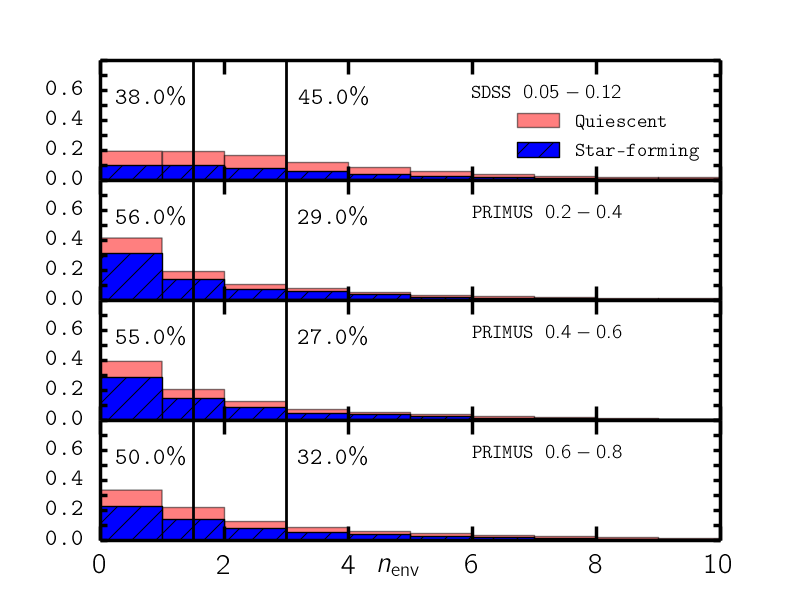
\epsfig{file=fig_envcount_cylr2h25_thresh75_sdss_z0_05_0_12_primuszerr_masslimit_histogram.png,height=0.5\textwidth}
     \caption{Environment measure distribution for our galaxy sample.}      \label{fig:envcount}
    \end{center}
\end{figure*}

Using the low redshift SDSS-{\em GALEX} and intermediate redshift PRIMUS data described above, in this section, we define our galaxy sample which will be used to compute the SMFs and QFs. For PRIMUS, we begin with the selection criteria imposed in \cite{Moustakas:2013aa} for their parent sample. We take the statistically complete {\em primary} sample from the PRIMUS data (\cite{Coil:2011aa}) and impose magnitude limits on optical selection bands as specified in \cite{Moustakas:2013aa} Table 1. These limits are in different optical selection bands and have distinct values for the five PRIMUS target fields. We then exclude stars and broad-line AGN to only select objects spectroscopically classified as galaxies, with high-quality spectroscopic redshifts ($Q \geq 3$). In addition we impose a redshift range of $ 0.2 < z < 0.8$ for the PRIMUS galaxy sample, where $ z > 0.2$ is selected due to limitations from sample variance and $ z < 0.8$ is selected due to the lack of sufficient statistics in subsamples defined below. 

For the PRIMUS objects that meet the above criteria, we assign statistical weights (described in \cite{Coil:2011aa} and \cite{Cool:2013aa}) in order to correct for targeting incompleteness and redshift failures. The statistical weight, $w_i$, for each galaxy is given by
\begin{equation}
w_{i} = (f_{\rm{target}} \times f_{\rm{collision}} \times f_{\rm{success}})^{-1},
\end{equation}
Equation (1) in \cite{Moustakas:2013aa}. Given that our ultimate interest is in deriving the SMFs and QFs from our sample, we impose stellar mass limits in order to derive a stellar mass complete galaxy sample. 

Stellar mass completeness limits for a magnitude-limited survey such as PRIMUS is a function of redshift, the apparent magnitude limit of the survey, and the typical stellar mass-to-light ratio of galaxies near the flux limit. As done in \cite{Moustakas:2013aa}, we follow \cite{Pozzetti:2010aa} to empirically determine the stellar mass completeness limits. For each of the target galaxies we compute $\mathcal{M}_{\rm{lim}}$ using $\rm{log} \; \mathcal{M}_{\rm{lim}} = \rm{log} \; \mathcal{M} + 0.4 ( m - m_{\rm{lim}})$, where $\mathcal{M}$ is the stellar mass of the galaxy in $\mathcal{M_{\odot}}$, $\mathcal{M}_{\rm{lim}}$ is the stellar mass of each galaxy if its magnitude was equal to the survey magnitude limit, $m$ is observed apparent magnitude in the selection band, and $m_{\rm{lim}}$ is the magnitude limit for our five fields mentioned above. We construct a cumulative distribution of $\mathcal{M}_{\rm{lim}}$ for the $15\%$ faintest galaxies in $\Delta z=0.04$ bins. In each of these redshift bins, we calculate the minimum stellar mass that includes $95 \%$ of the galaxies. Separately for quiescent and star-forming galaxies, we fit quadratic polynomials to the minimum stellar masses versus redshift (galaxies are classified into star-forming or quiescent in the following section). Finally, we use the polynomials to obtain the minimum stellar masses at the center of redshift bins, $0.2-0.4$, $0.4-0.6$, and $0.6-0.8$, which are then used as PRIMUS stellar mass completeness limits.

To derive the low redshift portion of our galaxy sample, we start by limiting the SDSS-{\em GALEX} data to objects within $0.0375 < z < 0.145$, a redshift range later imposed on the volume-limited Environment Defining Population (Section \ref{sec:environment}). To account for the targeting incompleteness of the SDSS-{\em GALEX} sample, we use the statistical weight estimates provided by the NYU-VAGC catalog. Furthermore, to derive a stellar mass complete sample, we impose a uniform stellar mass limit of $10^9.8 \; \mathcal{M}_{\odot}$, which is determined from the mass-to-light ratio completeness limit of the SDSS-{\em GALEX} sample within the imposed redshift limit. 

With the stellar mass completeness limits above, we have a stellar mass complete sample derived from SDSS-{\em GALEX} and PRIMUS. However since our sample is derived from two different surveys, we must account for the disparity in the redshift uncertainty. While PRIMUS provides precise spectroscopic redshifts with $\sigma_{z}/(1+z) \approx 0.5 \%$, due to the higher redshift ranges it probes the uncertainties are significantly greater than that of the SDSS-{\em GALEX} redshifts. The differences in redshift uncertainties becomes especially important in environment classifications (environment measurements and classification is later discussed in Section \ref{sec:environment}). In order to have comparable contamination in environment classifications, we apply PRIMUS redshift uncertainties to our galaxy sample selected from SDSS-{\em GALEX}. For each SDSS-{\em GALEX} galaxy in our sample, we compute its $\sigma_z$ by randomly sampling within three standard deviations of a normal distribution where the standard deviation is derived from the $z_{\rm{SDSS}-GALEX}$ of the galaxy, $\sigma = 0.005 (1+z_{\rm{SDSS}- GALEX})$

The absolute magnitude ($M_{r}$) versus redshift for the galaxy sample (black squares) is plotted in Figure \ref{fig:targetEDP}. The left-most panel corresponds to the portion of the sample derived from the SDSS-{\em GALEX} data and the rest correspond to the target sample derived from the PRIMUS data divided in bins with $\Delta z \sim 0.2$. 

\subsection{Classifying Quiescent and Star-Forming Galaxies} \label{sec:sfq}
With the galaxy sample defined in the previous section, we now classify the galaxies as quiescent or star-forming using an evolving cut based on specific star-formation rate utilized in \cite{Moustakas:2013aa} Section 3.2. This classification method utilizes the star-forming (SF) sequence, which is the correlation between star-formation rate (SFR) and stellar mass in star-forming galaxies observed at least until $z \sim 2$ (\cite{Noeske:2007aa}). The PRIMUS sample displays a well-defined SF sequence within the redshift range of our galaxy sample. Then using the power-law slope for the SF sequence derived by \cite{Salim:2007aa} (SFR $\propto \mathcal{M}^{0.65}$) and the minimum of the quiescent/star-forming bimodality, determined empirically, we obtain the following equation to classify the target galaxies (Equation 2 in \cite{Moustakas:2013aa}):
\begin{equation}
\rm{log}(\rm{SFR}_{\rm{min}}) = -0.49 + 0.64 \rm{log}(\mathcal{M} - 10) +1.07(z-0.1), 
\end{equation} \label{eq:qsfclass} 
where $\mathcal{M}$ is the stellar mass of the galaxy. If the target galaxy SFR and stellar mass lies above Equation \ref{eq:qsfclass} we classify it as star-forming; if below, as quiescent (\cite{Moustakas:2013aa} Figure 1.).

\begin{figure*}
  \begin{center}
    \leavevmode
    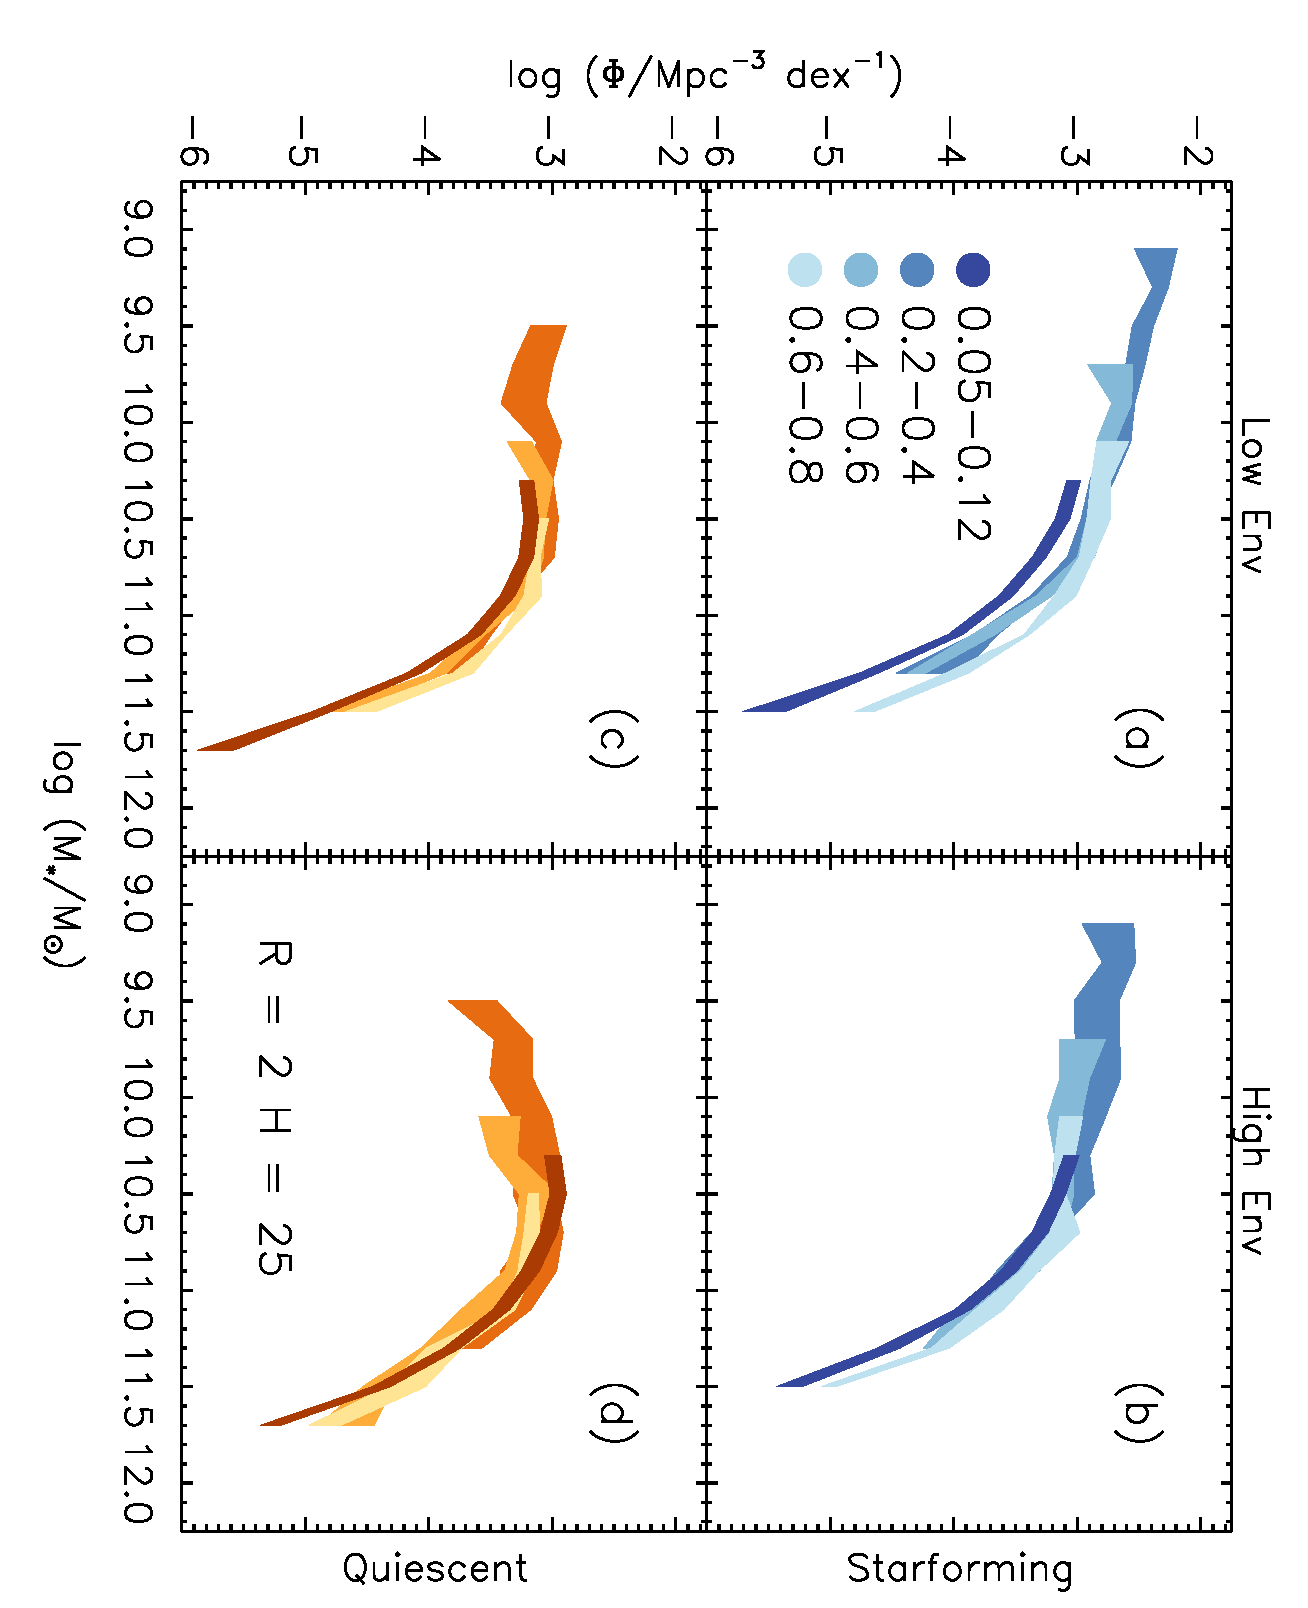
\epsfig{file=fig_smf_cylr2h25_thresh75_bin0_20_sdss_z0_05_0_12_primus_z0_2_1_0_lit_2envbin_primuszerr.eps,height=0.75\textwidth,angle=90}
     \caption{Evolution of stellar mass functions of star-forming (top) and quiescent (bottom) target galaxies in 
low (left) and high (right) environments from redshift range $z=0-0.8$. The environment of each galaxy  
was calculated using a cylindrical aperture size of $R=2 \: \rm{Mpc}$ and $H=25 \: \rm{Mpc}$ and  
classification based on the cut-offs specified in Table \ref{tab:aperture}. The SMFs use mass bins of 
width $\Delta \rm{log}(\mathcal{M}/\mathcal{M}_{\odot})=0.25$. In each panel we use shades of blue 
(star-forming) and orange (quiescent) to represent the SMF at different redshift, higher redshifts being
progressively lighter.}      \label{fig:smf}
    \end{center}
\end{figure*}

\subsection{Galaxy Environment} \label{sec:environment}
With the galaxy sample divided into quiescent and star-forming galaxies above, we now classify the galaxies into high and low density environments. In this section, we describe our method for measuring the environment for our galaxy sample. First, we define the environment of a galaxy as the number of neighboring {\em Environment Defining Population} galaxies (defined below) within a fixed aperture centered around it. We use a fixed aperture measurement of environment because, as \cite{Muldrew:2012aa} finds in their comparison of different environment definition using simulations, it provides a better probe of the entire halo in comparison to other definitions of environment such as nearest neighbor, which provides a better tracer at inter-halo scales. For our aperture, we use a cylinder of dimensions: $R_{\rm{ap}} = 2 \; \rm{Mpc}/h$ and $H_{\rm{ap}} = 25 \; \rm{Mpc}/h$. Though spherical apertures are often used in literature (e.g. \cite{Croton:2005aa}), we use a cylindrical aperture in order to account for the PRIMUS redshift errors and redshift space distortions (i.e. "Finger of God" effect). \cite{Cooper:2005aa} finds that $\pm 1000 \; \rm{km} \; \rm{s^{-1}}$ optimally reduces the effects of redshift space distortions and the PRIMUS redshift uncertainty at $z \sim 0.7$ corresponds to $\sigma_z < 0.01$, so aperture height of $25 \; \rm{Mpc}/h$ accounts for both of these effects. Our choice of cylinder radius was motivated by scale dependence analyses in literature (\cite{Blanton:2006aa}, \cite{Wilman:2010aa}, and \cite{Muldrew:2012aa}), which suggest that galactic properties such as color and quenched fractions are dependent on halo-scale properties such as host dark matter halo mass. \cite{Wilman:2010aa}, which uses environment defined by annuli of different radii, find positive correlation for quenched fraction and color on scales $< 1 \; \rm{Mpc}$ and anti-correlation on scales $> 3 \; \rm{Mpc}$. Our choice of $2 \rm{Mpc}/h$ provides sufficient sample size of galaxies in dense environments, for robust statistics, while tracing galactic properties within the halo scale. When we extend our analysis to cylindrical apertures with $R_{\rm{ap}} = 1 \; \rm{Mpc}/h$, we find that the change does not qualitatively change our results (difference in $f_{Q} < 0.05$). 
%Similar fixed aperture methods have also been used in \cite{Croton:2005aa} for galaxies in the 2dF Galaxy Redshift 
%Survey (\cite{Colless:2003aa}) and in \cite{Muldrew:2012aa} for a mock galaxy catalogue generated from embedding 
%galaxies onto the Millenium Dark Matter Simulation (\cite{Springel:2005aa}). 

Using the fixed aperture environment definition, we now measure the environment for our galaxy sample. First, we construct a volume limited {\em Environment Defining Population} (EDP) with absolute magnitude cut-offs ($M_{r}$) at redshift bin of $\Delta z \sim 0.2$. The $M_{r}$ cut-offs for the EDP are selected such that the cumulative number density over $M_{r}$ for all redshift bins are equal. In addition to providing a reasonable comparison of environment measurements for wide redshift range, it also seeks to construct an EDP that contains similar galaxy populations through the redshift range (i.e. accounts for the progenitor bias). As \cite{Behroozi:2013aa} and \cite{Leja:2013aa} find in their analysis of the cumulative number density method, though it does not precisely account for the scatter in mass accretion or galaxy-galaxy mergers, it provides a reasonable means to compare galaxy populations over a wide range of cosmic time. 

In constructing the EDP for the PRIMUS (hereafter PRIMUS EDP) we use the same PRIMUS data used to select our galaxy sample (described in Section \ref{sec:target}). We restrict the PRIMUS galaxies to $0.2 < z < 0.8$ and divide them into bins of $\Delta z = 0.2$. Before we consider the cumulative number densities in these bins, we first determine the $M_r$ limit for the highest redshift bin ($0.6-0.8$) by examining the $M_{r}$ distribution with bin size $\Delta M_{r} = 0.25$ and select $M_{r,\rm{lim}}$ near the peak of the distribution where bins with $M_{r} > M_{r,\rm{lim}}$ have fewer galaxies than the bin at $M_{r, \rm{lim}}$. We conservatively choose $M_{r, \rm{lim}}(0.6 < z < 0.8)$ to be $M_{r} = -20.75$. Then for the lower redshift bins, we impose absolute magnitude limits ($M_{r,\rm{lim}}$) such that the cumulative number density of the bin ordered by $M_{r}$ is equal to the cumulative number density of the highest redshift bin at $M_{r, \rm{lim}}(0.6 < z < 0.8) = -20.75$. In these cumulative number density calculations, we account for the statistical weights of the galaxies (Section \ref{sec:primus} and \ref{sec:sdss}).

For the EDP of the SDSS-{\em GALEX} galaxy sample (hereafter SDSS EDP), we do not use the SDSS-{\em GALEX} parent data which uses the geometry of the combined angular selection function of the SDSS VAGC and {\em GALEX} (Section \ref{sec:sdss}). Instead, since FUV, NUV values are not necessary for EDP, we extend the parent data of the SDSS EDP to the entire SDSS VAGC, including galaxies outside of the {\em GALEX} window function. Furthermore, we impose a redshift range of $0.0375-0.145$ on the SDSS EDP. This redshift range was empirically determined to account for the lack of faint galaxies at $z \sim 0.2$ and the lack of bright galaxies at $z \sim 0.01$ in the SDSS VAGC. The lower bound was determined by the bright limit and the upper bound by the faint limit of the $M_r$ versus redshift distribution. As with the PRIMUS redshift bins, we determine the SDSS EDP $M_{r; \rm{lim}}$ by matching the cumulative number density of the highest redshift bin. We get $M_{r,\rm{lim}} = -20.57$, $-20.73$, $-20.80$ and $-20.95$ for the redshift bins $0.0375-0.145$, $0.2-0.4$, $0.4-0.6$, $0.6-0.8$, respectively. These absolute magnitude limits are illustrated in Figure \ref{fig:targetEDP}, which show clear $M_r$ cutoffs in the $M_{r}$ distribution versus redshift for the EDP (red circles) on top of the target galaxy sample (black). 

Finally we measure the environment for each galaxy in our sampling by counting the number of EDP galaxies, $n_{\rm{env}}$ with $RA$, $Dec$, and $z$ within our cylindrical aperture centered around it. Note that $n_{\rm{env}}$ accounts for the statistical weights of the EDP galaxies. Once we obtain environment measurements for all the galaxies in our galaxy sample, we classify galaxies with $n_{\rm{env}} < 1$ to be "low" environment density and galaxies with $n_{\rm{env}} > 3$ to be "high" environment densities. The high environment cutoff was selected in order to reduce contamination from galaxies in low environment densities while maintaining sufficient statistics. 

The analysis we describe below uses a fixed cylindrical aperture with dimensions $R_{\rm{ap}} = 2 \: \rm{Mpc}$ and $H_{\rm{ap}} = 25 \: \rm{Mpc}$ to measure environment; the same analysis was extended for varying aperture dimensions $R_{\rm{ap}} = 1, 2, 3 \: \rm{Mpc}$ and $H_{\rm{ap}} = 25, 50 \: \rm{Mpc}$. Minor adjustments to the environment classification thresholds were adopted in these analyses for the smaller apertures ($r_{\rm{ap}} = 0.5, 1 \rm{Mpc}$ and $r_{\rm{ap}} = 25 \rm{Mpc}$). The results obtained from using these different are consistent with the results later discussed in this paper. 

\begin{figure*}
    \begin{center}
        \leavevmode
        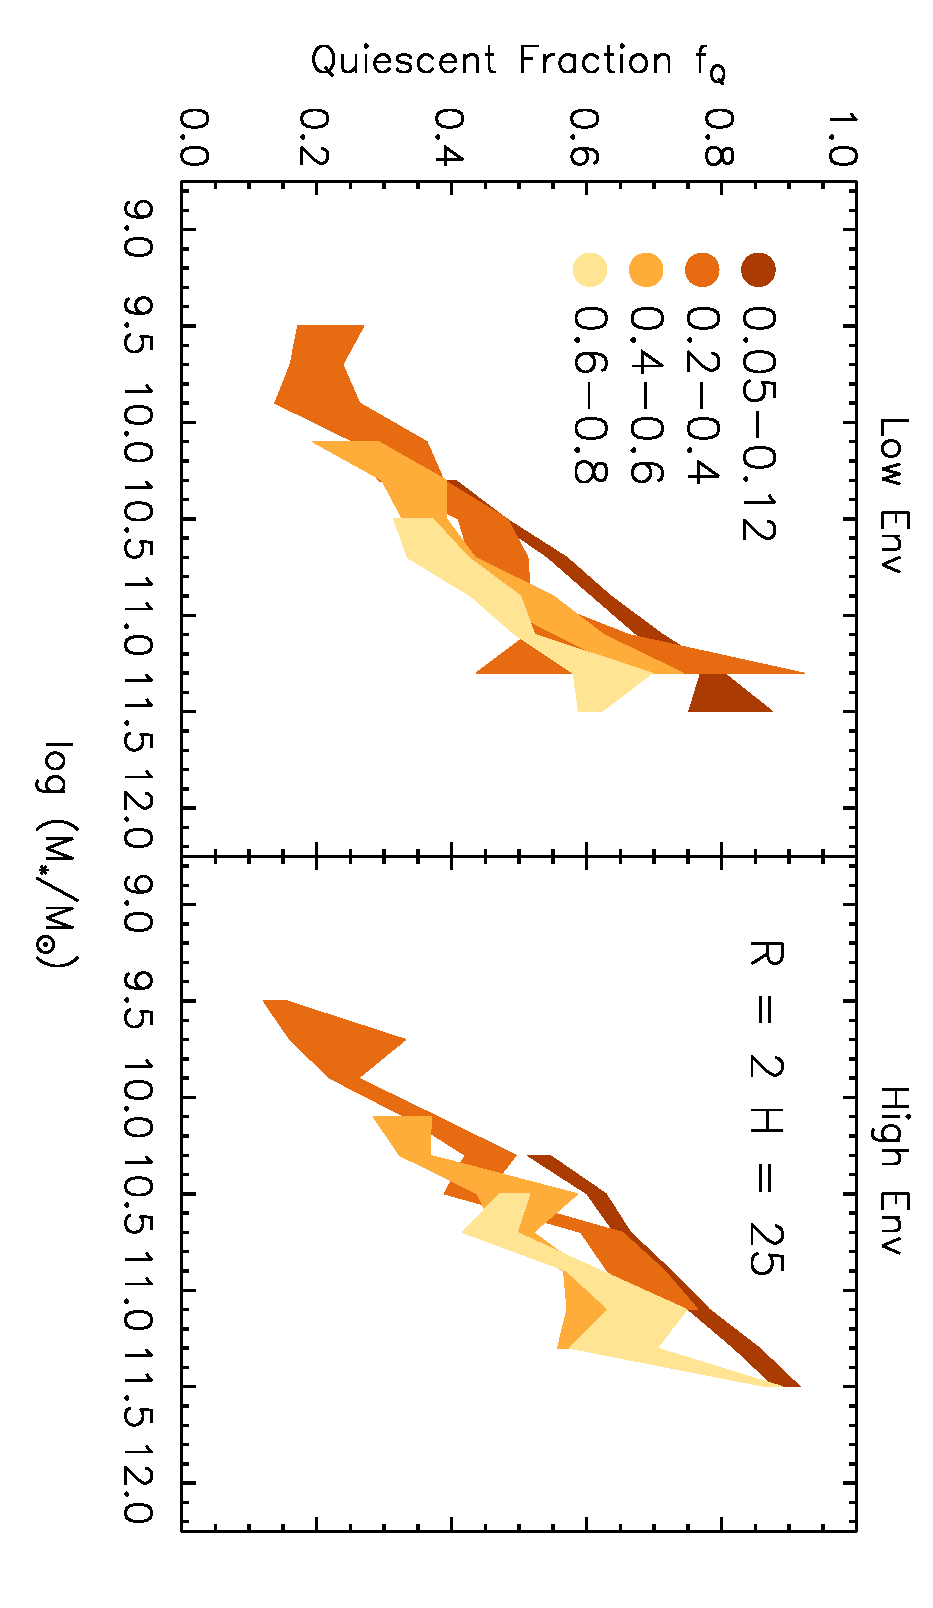
\epsfig{file=fig_qf_cylr2h25_thresh75_bin0_20_sdss_z0_05_0_12_primus_z0_2_1_0_lit_primuszerr.eps,height=0.75\textwidth,angle=90}
        \caption{Evolution of the quiescent fraction $f_{\rm{Q}}$ for galaxies in low (left) and high (rights) density environments for $z < 0.8$. $f_{\rm{Q}}$s were calculated using the SMFs in Figure\ref{fig:smf}, as described in text. Darker shading indicates lower redshift.}         \label{fig:qf}
    \end{center}
\end{figure*}

\subsection{Edge Effects} \label{sec:edgeeffect}
One of the challenges in obtaining accurate galaxy environments using a fixed aperture method is accounting for the edges of the survey. For galaxies located near the edge of the survey, part of the fixed aperture encompassing it will lie outside the survey regions. In this case, $n_{env}$ only reflects the fraction of the environment within the survey geometry.

To account for these edge effects, we use a Monte Carlo method to impose edge cutoffs on our galaxy sample. We begin by computing the angular separation, $\theta_{\rm{ap}}$ that corresponds to the radius of the fixed aperture (used to measure environment) at the redshifts of the galaxies. Then we compute the environment, $n_{\rm{ransack}}$, of our galaxy sample with the EDP replaced by a \texttt{ransack} sample of $N_{\rm{ransack}} = 1,000,000$ points with $RA$ and $Dec$ randomly selected within the window function of the EDP. We compare the $n_{\rm{ransack}}$ values to the expected value computed based on the angular area of the environment defining aperture and the EDP window function: 
\begin{equation} \label{eq:ransack}
E[n_{\rm{ransack}}] = \frac{N_{\rm{ransack}}}{A_{\rm{EDP}}}\times {\pi \theta_{\rm{ap}}^2} \times f_{\rm{thresh}}. 
\end{equation} 
$A_{\rm{EDP}}$ is the total angular area of the EDP window function and $f_{\rm{thresh}}$ is the fractional threshold for the edge effect cut-off, which we vary based on $R_{\rm{ap}}$ (listed in Table \ref{tab:aperture}). If $n_{\rm{ransack}}$ for a target galaxy is greater than $E[n_{\rm{ransack}}]$ then the galaxy remains in our sample; otherwise, it is discarded. 

\section{Stellar Mass Function} \label{sec:smf}
The target galaxy sample defined above has so far been classified into quiescent or star-forming and low or high density environments. We further divide these subsamples into redshift bins: $0.0375-0.145$, $0.2-0.4$, $0.4-0.6$, and $0.6-0.8$ for a total 16 subsamples. In this section, we calculate the SMF for each of these subsamples. 

To calculate the SMFs we employ a non-parametric $1/{V_{\rm{max}}}$ estimator commonly used for galaxy luminosity functions and stellar mass functions, as done in \cite{Moustakas:2013aa} and discussed in the review \cite{Johnston:2011aa}. The differential SMF is given by the following equation:
\begin{equation} \label{eq:phi}
\Phi(\rm{log}\: \mathcal{M}) \Delta(\rm{log} \:\mathcal{M}) = \sum\limits_{i=1}^{N} \frac{w_i}{V_{\rm{max,avail},i}}. 
\end{equation}
The equation above is same as Equation 3. in \cite{Moustakas:2013aa} except that we use $V_{\rm{max,avail}}$ instead than $V_{\rm{max}}$, to account for the edge effects of the survey discussed in Section \ref{sec:edgeeffect}. $w_i$ is the statistical weight of galaxy $i$ and $\Phi(\rm{log}\: \mathcal{M}) \Delta(\rm{log}\: \mathcal{M})$ is the number of galaxies ($N$) per unit volume within the stellar mass range $[\rm{log} \:\mathcal{M}, \rm{log} \:\mathcal{M}+\Delta(\rm{log} \:\mathcal{M})]$.

$V_{\rm{max},i}$ is the maximum cosmological volume where it is possible to observe galaxy $i$ given the apparent magnitude limits of the survey. However in Section \ref{sec:edgeeffect} we remove galaxies that lie on the edge from our sample. In doing so we reduce the maximum cosmological volume where a galaxy can be observed, thereby reducing $V_{\rm{max},i}$. We introduce the term $V_{\rm{max,avail},i}$ for the $V_{\rm{max},i}$ value that accounts for the survey edge effects. 

To calculate $V_{\rm{max,avail},i}$, we generate a sample of points with random $RA$, $Dec$ within the window function of our galaxy sample (SDSS-{\em GALEX} window function and the five PRIMUS fields) and random $z$ within the redshift range. This is not to be confused with the \texttt{ransack} sample in Section \ref{sec:edgeeffect}. We then impose the same edge effect cutoffs we applied to our galaxy sample, using the same \texttt{ransack} environment calculation method, also discuseed in Section \ref{sec:edgeeffect}. At redshift bins of $\Delta z \sim 0.01$, we compute the fraction of random points that remain in the bin after the edge effect cutoffs: $f_{\rm{edge}}$. We then apply this factor to compute $V_{\rm{max,avail}} = V_{\rm{max}} \times f_{\rm{edge}}$. The $V_{\rm{max}}$ in the equation above are computed following the method described in \cite{Moustakas:2013aa} Section 4.2 with the same redshift-dependent $K$-correction from observed SED and luminosity evolution model.

In order to calculate the uncertainty of the SMFs from the sample variance, we use a standard jackknife technique (as done in \cite{Moustakas:2013aa}). For the PRIMUS galaxies, we calculate SMFs after excluding one of the five target fields at a time. For the SDSS target galaxies we divide the field into a 12 $\times$ 9 rectangular $RA$ and $Dec$ grid and calculate the SMFs after excluding one grid each time. Using the calculated SMFs we calculate the uncertainty: 
\begin{equation}
\sigma^j = \sqrt{\frac{M-1}{M} \sum\limits_{k=1}^{M} (\Phi^j_k - \langle \Phi^j \rangle)^2}
\end{equation} 
$M$ in this equation is the number of jack knife SMFs in the stellar mass bin. $\langle \Phi^j \rangle$ is the mean number density of galaxies 
in each stellar mass bin for all of the jack knife $\Phi^j$s. 

In Figure \ref{fig:smf}, we present the SMFs for 16 target galaxy subsamples classified into quiescent/star-forming (orange/blue, bottom/top panels) and high/low environment density (left/right panels). The redshift evolution of the SMFs in each of these panels are indicated by a darker shade for lower redshift bins. The sample variance uncertainties are illustrated through the width of the SMFs. 

Although we imposed PRIMUS redshift errors on our SDSS galaxies in order to consistently measure environment throughout our entire sample, we observe a significant discrepancy between the SDSS and PRIMUS samples in the fractional contribution of each environment classification within the redshift bin. For each of the PRIMUS redshift bins, approximately $50 \%$ of galaxies in the redshift bin are in low density environments and roughly $30 \%$ are in high density environments. In contrast, in the SDSS redshift bin, $38 \%$ of galaxies in the redshift bin are in low density environments and $45 \%$ are in high density environments. As a result, we caution that the SMF redshift evolution is inconsistent during the transition from the PRIMUS sample to the SDSS sample at $z \sim 0.2$. 

Yet, from the PRIMUS samples alone, we probe a sufficient redshift to observe notable trends in the SMF evolution for each of the panels in Figure \ref{fig:smf}. Later we compare these trends to SMF results from DEEP2 (\cite{bundy06a}) and zCOSMOS (\cite{Bolzonella:2010aa}). In panel (a), star-forming galaxies in low density environments, we find a significant decrease in the high mass end of the SMF ($\mathcal{M} > 10^{10.75} \mathcal{M}_{\odot}$). In contrast at lower masses ($\mathcal{M} < 10^{10.5} \mathcal{M}_{\odot}$) we observe a notable increase in the SMF. In panel (b), star-forming galaxies in high density environments, we notice a possible decrease above the knee of the SMF ($\mathcal{M} \sim 10^{10.7} \mathcal{M}_{\odot}$) accompanied by an increase below the knee. For the quiescent population in low density environment, shown in panel (c) of Figure \ref{fig:smf}, we notice an increase in $\Phi$ for lower masses, but we do not notice any clear SMF evolution at the massive end. Lastly for the quiescent population in high density environments, panel (d), we find significant increase in $\Phi$ at all masses. 

In comparison to \cite{bundy06a} and \cite{Bolzonella:2010aa}, some of the noted trends are not immediately evident. However, this is mostly due to the conflicting mass limits proposed in each study. Not to mention, only part of the redshift range probed by \cite{bundy06a} overlap with our results. Overall, we find that the trends we note in the SMF evolution above are in good agreement with results from DEEP2 and zCOSMOS. 

Observing the evolutionary trends in SMF for each of these sub-populations simultaneously provides a naive narrative of the different galaxy evolutionary tracks involving environment and quenching. For example, the decrease in the massive star-forming galaxies in low density environment over cosmic time can be attributed to the transition of those galaxies to any of the other panels. The star-forming galaxies in low density environments that have quenched their star formation over time are possibly responsible for the increase of the quiescent, low density environment SMF over time. The star-forming galaxies that fall into higher density environments explain the increase in the star-forming high density environment SMF below the knee. Finally, star-forming galaxies in high density environments that have quenched their star-formation, quiescent galaxies that have transitioned from low to high density environments, and star-forming galaxies in low density environments that quench their star-formation while infalling to high density environments all contribute to the overall increase of the high environment quiescent SMF.

In addition to the evolution over cosmic time, we observe noticeable trends when we compare the SMFs for star-forming and quiescent galaxies between the two environments. Comparison of the SMFs in low versus high density environments reveal a noticeable relation between mass and density, with SMFs in high density environments having more massive galaxies. We further confirm this trend when we compare the median mass between the two environments to find that the median mass for galaxies in high density environments is significantly greater than in low density environments. The relationship between mass and environment observed in our SMFs mirror the well-established mass-density relation and observed mass segregation with environment in the literature (\cite{bundy06a}; \cite{Scodeggio:2009aa}; \cite{Bolzonella:2010aa}).

We caution readers and reserve detailed analysis of the SMFs to future work due to the improvements in photometry that significantly alter the SDSS SMFs mentioned in Section \ref{sec:sdss}. 
% There is also the issue with the SMF evolution: the uneven fractional contribution of the population and each environment classification. 

\section{Quiescent Fraction} \label{sec:qf_const}
The SMFs calculated in the previous section illustrate the stellar mass distribution of our galaxy population and its evolution over comic time. In this section, using the SMFs of our subsamples, we compare the quiescent and the star-forming populations by calculating the fraction of galaxies that have quenched their star-formation, the quiescent fraction. With the sufficient statistics available from SDSS and PRIMUS, we evaluate the quiescent fraction in bins of stellar mass and redshift for low and high density environments. More specifically, by analyzing the quiescent fraction with respect to mass, redshift, and environment we are able to compare the quiescent fraction evolution in low and high density environments. Through this comparison we reveal the subtle environmental effects in quenching star formation that are often obscured by the underlying correlations among galactic properties such as color-mass and mass-density relations (\cite{Cooper:2010aa}). Furthermore by quantifying the environmental effects of star-formation quenching, we are able to provide constraints on the various proposed environmental quenching mechanisms, such as strangulation and ram-pressure stripping (\cite{McCarthy:2008aa}).

From the SMF number densities ($\Phi$) computed in the previous section, the quiescent fraction is computed as follows, 
\begin{equation}
f_{\rm{Q}} = \frac{\Phi_{Q}}{\Phi_{SF}+\Phi_{Q}}.
\end{equation}
$\Phi_{Q}$ and $\Phi_{SF}$ are the total number of galaxies per unit volume in stellar mass bin of $\Delta(\rm{log} \: \mathcal{M}) = 0.25$ for the quiescent and star-forming subsamples, respectively (Equation \ref{eq:phi}). We compute $f_{\rm{Q}}$ for high and low density environments for all redshift bins as plotted in Figure \ref{fig:qf}, which shows the evolution of $f_{\rm{Q}}$ for high (right) and low (left) density environments. As in Figure \ref{fig:smf}, the darker shading represent lower redshift bins. 

Most noticeably in Figure \ref{fig:qf}, $f_{\rm{Q}}$ increases monotonically as a function of mass at all redshift bin and environment. In other words, for all subsamples, galaxies in higher mass bins are more likely to have quenched its star-formation. With the roughly linear correlation between galaxy SFR to galaxy color and morphology, we find that this trend reflects the well established color-mass and morphology-mass relations: more massive galaxies are more likely to be red or early-type (\cite{blanton09a}). 

Focusing on the redshift evolution of $f_{\rm{Q}}$, we find that for both environments $f_{\rm{Q}}$ increases as redshift decreases. For high density environment, this is analogous to the Butcher-Omeler Effect (\cite{Butcher:1984aa}), which states that galaxy populations in groups or clusters have higher $f_{\rm{blue}}$, or lower $f_{\rm{Q}}$, at higher redshift. For all environments a larger portion of our galaxy population has quenched its star-formation over time. Coupled with the decline of SFR in the star-forming population (\cite{Noeske:2007aa}; \cite{cooper08a}), our results strongly agree with the observed decline of global star-formation in the universe (\cite{hopkins06a}). %Maybe Stacey et al. 2014 is relevant here? 

In addition, when we compare the stellar masses at which $f_{\rm{Q}} = 0.5$ for each subsample, we find that this mass decreases over cosmic time. This corresponds to the well-known mass-downsizing pattern in the literature (e.g. \cite{bundy06a}). Furthermore, the mass-downsizing trend observed in each of our environment subsample is consistent with the trend observed in zCOSMOS Redshift Survey for isolated and group galaxies (\cite{Iovino:2010aa}). %Remark on how the M_{50-50}? is lower for high environment f_{Q}, and that it generally increases with redshift. A trend also observed in the t_{5050} considerations.

Finally, we compare our $f_{\rm{Q}}$ results to previous $f_{\rm{Q}}/f_{\rm{red}}$ measurements for analogous environment classifications. For our lowest redshift bin, we find that our $f_{\rm{Q}}$ values for low and high environments are consistent with previous $f_{\rm{Q}}/f_{\rm{red}}$ measurements for SDSS galaxies as a function of environment. For example, \cite{Tinker:2011aa}, using a group-finding algorithm on the SDSS DR7, presents the relationship between $f_{\rm{Q}}$ and overdensity for galaxies within the mass range $\rm{log} \; \mathcal{M} = [9.8, 10.1]$. The \cite{Tinker:2011aa} $f_{\rm{Q}}$ at the lowest and highest overdensities, $f_{\rm{Q}} \sim 0.4$ and $f_{\rm{Q}} \sim 0.6$ respectively, are consistent with our $f_{\rm{Q}}$ for low and high density environment at the lowest mass bin ($\rm{log} \; \mathcal{M} \sim 10.2$). At higher masses, our $f_{\rm{Q}}$ results are consistent with \cite{Baldry:2006aa}. \cite{Baldry:2006aa} uses project neighbor density environment measures ($\rm{log} \;  \Sigma$) to obtain $f_{\rm{Q}}(\mathcal{M})$ for a range of environmental densities. Although the different environment measurements make a direct comparison unclear, at higher environments ($\rm{log} \; \Sigma > 0.2$) in \cite{Baldry:2006aa} $f_{\rm{Q}} \sim 0.6$ at $\mathcal{M} \sim 10^{10.2} \mathcal{M}_{\odot}$ and $f_{\rm{Q}} \sim 0.9$ at $\mathcal{M} \sim 10^{11.5} \mathcal{M}_{\odot}$, in agreement our high density environment. Likewise, for lower environments in \cite{Baldry:2006aa} ($\rm{log} \; \Sigma < -0.4$) $f_{\rm{Q}} \sim 0.4$ at $\mathcal{M} \sim 10^{10.2} \mathcal{M}_{\odot}$ and $f_{\rm{Q}} \sim 0.8$ at $\mathcal{M} \sim 10^{11.5} \mathcal{M}_{\odot}$, which also agree with our low density environment $f_{\rm{Q}}$. 

For $z > 0.2$, we compare our PRIMUS $f_{\rm{Q}}$ results to the $f_{\rm{red}}$ (or $1-f_{\rm{blue}}$) results from the zCOSMOS Redshift Survey (\cite{Iovino:2010aa}, \cite{Cucciati:2010aa}, \cite{Kovac:2014aa}), which approximately covers the same redshift range as PRIMUS. \cite{Iovino:2010aa}, \cite{Cucciati:2010aa}, and \cite{Kovac:2014aa} using a mass-complete galaxy sample derived from zCOSMOS and a group catalog, 3D local density contrast, and overdensity environment measurements, respectively, compare $f_{\rm{red}}$ with respect to environment. The $f_{\rm{blue}}$ for group and isolated galaxies from \cite{Iovino:2010aa} are generally inconsistent with our $1-f_{\rm{Q}}$ for high and low density environments. Similarly, $f_{\rm{red}}$ for high and low overdensities in \cite{Kovac:2014aa} are  greater overall than the PRIMUS $f_{\rm{Q}}$ values in high and low density environments. However, \cite{Kovac:2014aa} points out that there is a significant difference between classifying the quenched population using color and SFR. $f_{\rm{Q}}$ defined by color is greater than $f_{\rm{Q}}$ defined by SFR by roughly $0.2$. Although the propagation of this difference for different environments is not explored in \cite{Kovac:2014aa}, if we account for the difference evenly for $f_{\rm{red}}$ at all environments, the \cite{Kovac:2014aa} results are generally consistent with our $f_{\rm{Q}}$ at high and low density environments. 

Additionally, the zCOSMOS results indicate that the $f_{\rm{red}}$ values in high density environments are greater overall than in low density environments. The same trend is observed in the PRIMUS results and will be discussed in detail later in the section. Another significant trend observed in the zCOSMOS results is the significant mass dependence of the $f_{\rm{red}}$ and $f_{\rm{blue}}$ evolution. \cite{Iovino:2010aa} by examining $f_{\rm{blue}}(z)$ in different mass bins for group and isolated galaxies find significantly larger $f_{\rm{blue}}$ evolution at lower masses. In fact, \cite{Iovino:2010aa} finds no evolution in $f_{\rm{blue}}$ for $\mathcal{M} > 10^{10.9} \mathcal{M}_{\odot}$ for both group and isolated galaxies over the redshift range $0.4 < z < 0.9$. On the other hand, in the lowest mass bin ($10^{10.0} \mathcal{M}_{\odot} < \mathcal{M} < 10^{10.5} \mathcal{M}_{\odot}$) \cite{Iovino:2010aa} finds $f_{\rm{blue}}(z \sim 0.4) - f_{\rm{blue}}(z \sim 0.2) \sim 0.2$ for isolated galaxies and  $f_{\rm{blue}}(z \sim 0.4) - f_{\rm{blue}}(z \sim 0.2) \sim 0.1$ for group galaxies. In contrast, in each of the panels of Figure \ref{fig:qf}, we qualitatively find little mass dependence on the $f_{\rm{Q}}$ evolution for either low or high density environments. However, due to the distinct stellar mass completeness limits imposed at each redshift bin of our sample, subtle effects such as the mass dependence of the $f_{\rm{Q}}$ evolution are difficult to discern. 

In order to more quantitatively compare the $f_{\rm{Q}}$ evolution, we fit $f_{\rm{Q}}$ for each subsample to a power-law parameterization as a function of stellar mass, 
\begin{figure}
    \begin{center}
        \leavevmode
        \epsscale{1.0}
        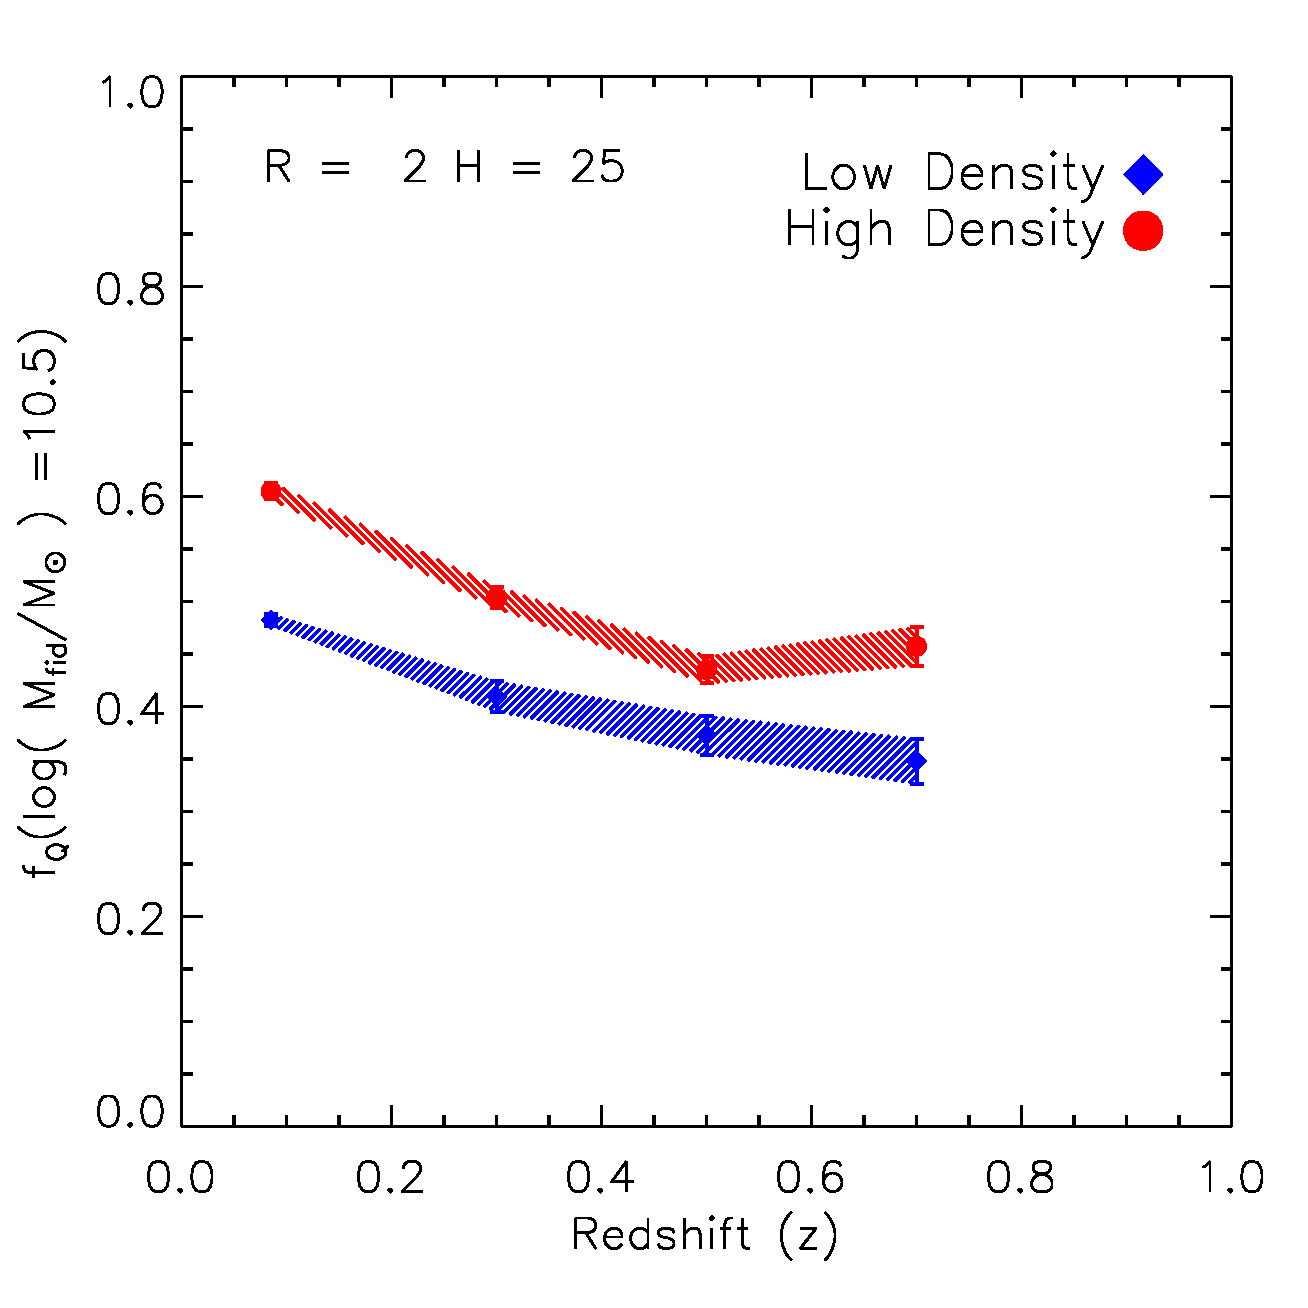
\epsfig{file=fig_qffit_cylr2h25_thresh75_bin0_20_sdss_z0_05_0_12_primus_z0_2_1_0_fidmass10_5_lit_primuszerr.eps,height=0.45\textwidth}
        \caption{The evolution of the quiescent fraction at fiducial mass, $f_{Q}(\mathcal{M}_{\rm{fid}} = 10^{10.5} \mathcal{M}_\odot)$, for low (square) and high (circle) density environments within the redshift range $z = 0.0 - 0.8$.  There is a significant increase in $f_{Q}(\mathcal{M}_{\rm{fid}})$ with decrease in redshift for both environments. In addition, over the entire redshift range, high density environment $f_{Q}(\mathcal{M}_{\rm{fid}})$ is greater than low density environment $f_{Q}(\mathcal{M}_{\rm{fid}})$. However the difference in $f_{Q}(\mathcal{M}_{\rm{fid}})$ for the two environments remains constant throughout suggesting that while the quiescent fraction is higher in dense environments, the evolution of the quiescent fraction is independent of environment.}         \label{fig:qffit}
    \end{center}
\end{figure}

\begin{equation} 
f_{\rm{Q}}(\mathcal{M}_{*}) = a \: \rm{log} \; \left(\frac{ \mathcal{M}_{*}}{10^{10.5} \: \mathcal{M}_{\odot}} \right)+b,
\end{equation}
where $a$ are $b$ are best-fit parameters using {\em MPFIT} (\cite{Markwardt:2009aa}). The value $10^{10.5} \: \mathcal{M}_{\odot}$ in the equation represents an empirically selected fiducial mass $\mathcal{M}_{\rm{fid}}$ within the stellar mass limits where there is a sufficiently large number of galaxies. This fiducial mass serves to highlight and quantify the $f_{\rm{Q}}$ evolution for different redshifts. Figure \ref{fig:qffit} shows the evolution of $f_{\rm{Q}}(\mathcal{M}_{\rm{fid}})$ from $z \sim 0.7$ to $\sim 0.1$ for low (diamond) and high (circle) density environments. 

Figure \ref{fig:qffit} illustrates that throughout the entire redshift range, high density environment has a significantly greater $f_{\rm{Q}}(\mathcal{M}_{\rm{fid}})$ than the lower density environment. This is in strong agreement with the zCOSMOS results from \cite{Cucciati:2010aa} and \cite{Kovac:2014aa}. For $z < 1.0$, galaxy populations in higher density environments have higher quenched fractions. As galaxy color and SFR are related, our results support the existence of the color-density relation (\cite{Cucciati:2010aa}; \cite{Cooper:2010aa}) in favor of the idea that the color-density relation is a merely a reflection of the mass-density or morphology-density relation (\cite{Scodeggio:2009aa}, \cite{Tasca:2009aa}).  

The same fitting procedure was performed using $\mathcal{M}_{\rm{fid}} = 10^{11} \mathcal{M}_\odot$; however, aside from an overall shift in $f_{\rm{Q}}(\mathcal{M}_{\rm{fid}})$ by $\sim 0.2$, we observe the same evolutionary trends. $f_{\rm{Q}}(\mathcal{M}_{\rm{fid}} = 10^{11}\mathcal{M}_{\odot})$ for both low and high density environments each increase by $\sim 0.2$ as redshift decreases from $\sim 0.7$ to $\sim 0.1$, just as Figure \ref{fig:qffit}. Evidently, increasing the fiducial mass to $10^{11} \mathcal{M}_{\odot}$ does not change the total evolution for either environments. On the other hand, \cite{Iovino:2010aa}, for both group and isolated galaxies, finds significantly less $f_{\rm{Q}}$ evolution for $\mathcal{M} \sim 10^{11.0} \mathcal{M}_{\odot}$ than in $\mathcal{M} \sim 10^{10.5} \mathcal{M}_{\odot}$. Furthermore, \cite{Iovino:2010aa} also finds that the difference in $f_{\rm{blue}}$ evolution between group and isolated galaxies ($f_{\rm{blue}, \rm{isolated}}(z) - f_{\rm{blue}, \rm{group}}(z))$ is much greater at $\mathcal{M} \sim 10^{10.5} \mathcal{M}_{\odot}$ than at $\mathcal{M} \sim 10^{11} \mathcal{M}_{\odot}$, where they find almost no difference. In contrast, we find that changing the fiducial mass does not significantly alter the difference in $f_{\rm{Q}}(\mathcal{M}_{\rm{fid}})$. The zCOSMOS results find a clear mass dependence in the $f_{\rm{blue}}$ evolution; however, the consistency in evolutionary trends when the fiducial mass is change reveal that our $f_{\rm{Q}}$ evolution exhibits little mass dependence. Although our sample from SDSS and PRIMUS provides significantly larger statistics, due to the limited mass ranges probed in our mass-complete sample (e.g. $\mathcal{M} > 10^{10.5} \mathcal{M}_{\odot}$ for our $z \sim 0.7$ bin) it is difficult to dismiss the mass dependence observed in the zCOSMOS results.

Finally, from Figure \ref{fig:qffit}, we note that for both environments $f_{\rm{Q}}(\mathcal{M}_{\rm{fid}})$ increases as redshift decreases. This highlights the general increase of $f_{\rm{Q}}(\mathcal{M})$ as redshift decreases noted earlier. More importantly, we quantify the total evolution of $f_{\rm{Q}}$ for both low and high density environments through $f_{\rm{Q}}(\mathcal{M}_{\rm{fid}}, z \sim 0.1) - f_{\rm{Q}}(\mathcal{M}_{\rm{fid}}, z \sim 0.7)$ for both environments. Remarkably, $f_{\rm{Q}}$ evolves by the same amount for both environments. In other words, the total evolution of $f_{\rm{Q}}(\mathcal{M}_{\rm{fid}})$ from $z \sim 0.7$ to $\sim 0.1$ show little environment dependence. This disagrees with the $f_{\rm{blue}}$ results from \cite{Iovino:2010aa}, which show a clear distinction between group and isolated galaxies. In \cite{Iovino:2010aa}, $f_{\rm{blue}}$ for isolated galaxies decrease much faster than $f_{\rm{blue}}$ for group galaxies. At $\mathcal{M} \sim 10.5$, \cite{Iovino:2010aa} finds that $f_{\rm{blue}}$ for isolated galaxy decreases by 0.3 from $z \sim 0.6$ to 0.3, while for $f_{\rm{blue}}$ for group galaxies only decrease by 0.1 in the same redshift limit, showing a clear dependence in environment. Considering that fixed aperture definition of environment is susceptible to contamination due to PRIMUS redshift errors, we consider more stringent classification of high density environments extending the cut-off to $n_{\rm{env}} > 6, 9$. While a more stringent classification increases the $f_{\rm{Q}}(\mathcal{M}_{\rm{fid}})$ overall as well as the uncertainties, it does not reveal reveal any significant environment dependence in the $f_{\rm{Q}}$ evolution. Therefore, the potential contamination in our environment measurements cannot explain the lack of environment dependence in the $f_{\rm{Q}}$ evolution. 

Many physical mechanisms have been proposed to explain the quenching of star-formation observed in our universe. Often star-formation quenching is classified into two distinct mechanisms: mass-dependent and environment dependent mechanisms (\cite{Baldry:2006aa}; \cite{Peng:2010aa}). From the mass-dependence presented in all $f_{\rm{Q}}$ in Figure \ref{fig:qf}, we concur that galaxy stellar mass plays a significant role in quenching. Furthermore, since $f_Q$ in high density environments is always greater than $f_Q$ in low density environments, our results also reflect the environment dependence in quenching. %However, in many of the proposed environment dependent quenching mechanisms, the quenching time scale is proposed to decrease. This would result in an increase in the quenched fraction that's faster than the increase in low density environment $f_Q$. We find that this is not the case. % What does this have to say about physical processes in groups and clusters that affect quenching?

\section{Summary} \label{sec:summary}
Using a stellar mass complete galaxy sampled derived from SDSS and PRIMUS accompanied by a consistently measured galaxy environment from robust spectroscopic redshifts, we measure the stellar mass functions for star-forming and quiescent in low and high density environments over the redshift range $z < 0.8$. From these stellar mass functions, we compare the proportion of quiescent galaxies within the subsamples by computing quiescent fraction for each of them. Afterwards, in order to better quantify the evolution of the quiescent fraction over cosmic time, we fit our quiescent fraction anchored at a fiducial mass. From our analyses we find the following notable results. 

\begin{enumerate}
	\item By noting the SMF evolution for each of our subsamples, we loosely trace the evolutionary tracks our galaxy population tracing the general evolutionary tracks of quenching mechanisms and galaxies infalling into high density environments. 
	\item From the SMFs, we find that our galaxy population in high density environments, both star-forming and quiescent, have a higher median mass, thus confirming the mass density relation and mass-segregation in different environments.
	\item In all of our subsamples, we find a clear mass dependence in $f_{\rm{Q}}$. $f_{\rm{Q}}$ increases monotonically with galaxy stellar mass. 
	\item Both from the $f_{\rm{Q}}$ evolution and $f_{\rm{Q}}(\mathcal{M}_{\rm{fid}})$ values, $f_{\rm{Q}}$ increases with redshift. 
	\item We conclude, by fitting our $f_{\rm{Q}}$, that $f_{\rm{Q}}$ in high density environments is greater than $f_{\rm{Q}}$ in low density environments regardless of mass and redshift. This result confirms the environmental dependence of quenching mechanisms stated previously in literature. 
	\item Comparison of the $f_{\rm{Q}}(\mathcal{M}_{\rm{fid}})$ evolution for high and low density environments that the total evolution is independent of environment. 
\end{enumerate}

%  demonstrate that the quiescent fraction increases over cosmic time for $ z < 0.8$, regardless of environment. During this epoch the quiescent fraction in high density environments is consistently greater than the quiescent fraction in low density environments. Furthermore, when we fit the quiescent fraction at a fiducial mass ($\mathcal{M}_{\rm{fid}}$), we find that the evolution of the quiescent fraction from $z \sim 0.8$ to $z \sim 0.1$ is similar for high and low density environments. 


We thank people...
%
% References
%
\bibliography{PRIMUS}

\appendix
\begin{table*} %Will contain much more information on environments. 
  \caption{Environment Defining Aperture Dimensions}
  \label{tab:aperture}
  \begin{center}
    \leavevmode
    \begin{tabular}{llllll} \hline \hline              
  Radius (Mpc)          &Height (Mpc)      & Edge Effect Cutoff &High Env (galaxies) &Low Env (galaxies) \\ \hline 
  1.0 &50 & 80\% & 1.5 & 0.0          \\
  2.0 &50 & 75\% & 4.0 & 0.0          \\ \hline
  \multicolumn{5}{l}{}                                             \\       
    \end{tabular}
  \end{center}
\end{table*}
\end{document}
